\section{Sistema de Tempo Real}
\label{sec:STR}

\subsection{Definição de um Sistema de Tempo Real}
\label{sec:DefSTR}
Um sistema de tempo real, ao contrário do que se costuma pensar, não tem
como objetivo uma execução necessariamente rápida, mas previsível.
Neste tipo de sistema, pode-se encontrar duas características fundamentais:

\begin{itemize}
\item Um sistema de tempo real precisa produzir resultados computacionais corretos
(chamados de correção lógica ou funcional).
\item Os resultados computacionalmente corretos obtidos precisam ser concluídos em
um período de tempo pré-definido, caracterizando a previsibilidade na execução da tarefa.
\end{itemize}

Sistemas de tempo real são definidos como sistemas nos quais a correção nos
resultados de execução de maneira geral são dependentes tanto da correção
lógica como da previsibilidade do tempo de execução, sendo assim, a previsibilidade
do tempo de execução é, ao menos, tão importante quanto a correção funcional
nesse tipo de sistemas.~\cite{Li:2003:RCE:829584}

Os sistemas de tempo real são utilizados para atender à tarefas que possuem algum tipo
de restrição temporal em sua execução. Esse tipo de necessidade está muito presente no
dia-a-dia, e são aplicados aos mais diversos tipos de tarefas, desde controladores de
leitores de DVDs, elevadores, freios de carro, controladores de mísseis até piloto automático
de aeronaves.

\subsection{Tipos de Sistema de Tempo Real}
Como abordado na seção~\ref{sec:DefSTR}, para que um sistema de tempo real obtenha uma
execução de tarefa correta, é necessário terminar essa execução em um período pré-definido,
chamado de \textit{deadline}. Portanto, é possível afirmar que este tipo de sistema, por possuir
essa restrição temporal, é regido pelos \textit{deadlines} de suas tarefas.

Devido a importância dos \textit{deadlines}, esse tipo de sistema pode ser classificado como
críticos ou não críticos, baseado na tolerância de \textit{deadlines} perdidos, a utilidade
dos resultados computados após a perda do \textit{deadline} e a severidade da penalidade em
perder um prazo de execução.

\subsubsection{Sistemas de Tempo Real Críticos}
Os sistemas de tempo real chamados de críticos são aqueles que possuem uma restrição severa
de prazo na execução de tarefas, ou seja, sua tolerância em perder prazos é muito pequena
ou nenhuma. Em muitos desses sistemas, as informações computadas fora do prazo são consideradas
inúteis, caracterizando uma penalidade grave em perder o prazo de execução.

Um sistema de tempo real crítico é um sistema que precisa executar suas tarefas dentro do prazo
pré-definido com uma tolerância muito próxima de zero. Os prazos devem ser atendidos, ou os resultados
são catastróficos. A perda de prazos na execução possui um custo muito alto, podendo inclusive
envolver vidas humanas. Os resultados computados após o prazo pré-definido possuem uma utilidade próxima
de zero ou possuem um grande grau de depreciação com a decorrência do tempo após o prazo.~\cite{Li:2003:RCE:829584} \\\\
Alguns exemplos de sistemas de tempo real considerados críticos são:
\begin{itemize}
\item Sistema de navegação de aeronaves.
\item Freios de carro (ABS).
\item Marca-passo.
\item Controladores de mísseis.
\end{itemize}

\subsubsection{Sistemas de Tempo Real Não Críticos}
Os sistemas de tempo real considerados não críticos são aqueles onde uma perda de prazo
resulta em uma penalidade leve, como uma distorção em uma música sendo lida de um CD, perda
de alguns frames em um vídeo entre outras consequências de baixa criticidade.

Esses sistemas precisam atender seus prazos pré-definidos, porém com um certo grau de flexibilidade.
Os prazos podem possuir diferentes graus de tolerância, prazos balizados com tempo médio e até em avaliação
estatística dos tempos de resposta. Nesse tipo de sistema, apesar da perda de prazos não resultar em uma
falha no sistema, os custos da perda dos mesmos pode se tornar grande, dependendo da proporção em que isso
ocorre.~\cite{Li:2003:RCE:829584} \\\\
Alguns exemplos de sistemas de tempo real considerados não críticos são:
\begin{itemize}
\item Sistema responsável por leitura de DVD.
\item Sistema de som em computadores pessoais.
\item Decodificador de sinal de televisão.
\end{itemize}

\subsection{HellfireOS}
\label{sec:HellfireOS}
O HellfireOS é um sistema operacional de tempo real altamente configurável que pode ser
utilizado tanto como um sistema de tempo real crítico como não crítico.
Projetado para sistemas MPSoC, possui gerenciamento dinâmico de tarefas que conta com a
proteção contra inversão de prioridades. Seu escalonador possui as seguintes políticas de escalonamento:

\begin{itemize}
\item Rate Monotonic
\item Round Robin
\item Earliest Deadline First
\item Deadline Monotonic
\end{itemize}

Seu mapeamento dinâmico de tarefas é feito através de primitivas para migração de tarefas, que pode
ser implícita ou explícita. Na migração explícita, o designer insere pontos de migração no código
da aplicação, já a migração implícita é feita por um mecanismo automatizado que monitora a carga do
sistema e envia ordem de migração para as tarefas. Geralmente, os benefícios da migração de tarefas são
o balanceamento de carga nos processadores, decréscimo no consumo de energia e suporte a técnicas de
tolerância a falhas.

HellfireOS é um micro-kernel portável composto de vários módulos e pode ser configurado de diversas maneiras,
ora visando o numero máximo de tarefas em um processador, ora definindo o tamanho da pilha da tarefa.
A ideia é permitir ao designer otimizar o tamanho final da imagem do kernel de acordo com as restrições
da aplicação e de sistema, permitindo assim que o designer possibilitem ao sistema rodar em plataformas com
baixa memória, como são os casos mais típicos de sistemas embarcados críticos.

Dentre as bibliotecas mais relevantes ao desenvolvimento da integração abordada na seção~\ref{sec:HAC},
constam uma LibC customizada e a biblioteca matemática (math.h) com emulação de número de ponto
flutuante. Outro ponto de interesse, nesse caso para a prova de conceito, é observarmos
que o HellfireOS não possui todas as camadas de rede implementadas, forçando a criação
ou das camadas faltantes, ou de outra solução, para possibilitar a integração.

A API do Hellfire é dividida em 5 (cinco) grupos:

\begin{itemize}
\item Manipulação de Tarefas
\item Exclusão Mútua
\item Manipulação de Memória
\item Comunicação entre Processos
\item LibC
\end{itemize}


\begin{figure}[H]
	\centering
		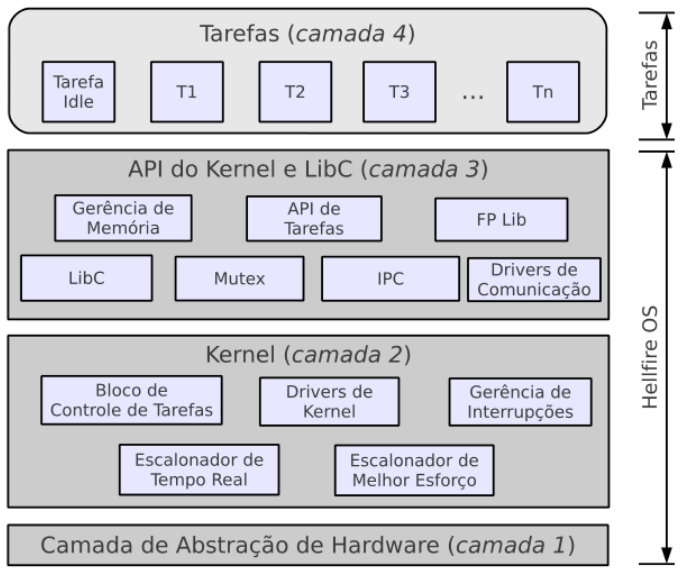
\includegraphics[width=0.5\textwidth]{fig/HellfireArch.png}
	\caption{Arquitetura em alto nível do HellfireOS.}
\end{figure}


O HellfireOS é parte constituinte do Hellfire System (HFS), que conta também com uma
plataforma para design que compreende diferentes níveis de abstração, partindo de aplicações
escritas em C até a prototipação em FPGAs. Isto é possível graças as ferramentas e módulos
que fazem parte do Hellfire Framework (HFFW).

O Hellfire Framwork apresenta um fluxo para o design de MPSoC baseado em sistemas embarcados do tipo crítico,
como equipamentos de uso médico, dispositivos de segurança e sistemas de aeronaves. Este tipo de sistema
apresenta uma necessidade específica de design, englobando preocupações especiais em relação ao consumo de
energia e alta performance, mantendo o processamento de tempo real~\cite{5450495}.
